% time values for run2, run6 and run7
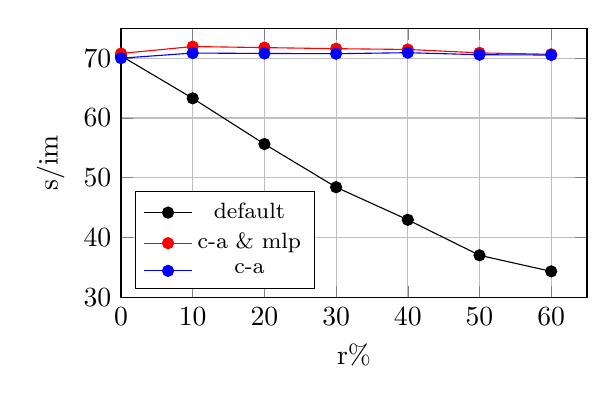
\begin{tikzpicture}
\begin{axis}[
    title={},
    height=5cm,
    width=7.5cm,
    xlabel={r\%},
    ylabel={s/im},
    xmin=0, xmax=65,
    ymin=30, ymax=75,
    xtick={0,10,20,30,40,50,60},
    ytick={30,40,50,60,70},
    legend pos=south west,
    xmajorgrids=true,
    ymajorgrids=true,
    legend style={font=\footnotesize}
]

\addplot[
    color=black,
    mark=*
    ]
    coordinates {
    (0,70.38)(10,63.28)(20,55.64)(30,48.42)(40,42.97)(50,37.04)(60,34.35)
    };
    
\addplot[
    color=red,
    mark=*
    ]
    coordinates {
    (0,70.78)(10,71.94)(20,71.76)(30,71.58)(40,71.45)(50,70.88)(60,70.64)
    };

\addplot[
    color=blue,
    mark=*
    ]
    coordinates {
    (0,69.99)(10,70.85)(20,70.78)(30,70.74)(40,70.91)(50,70.57)(60,70.52)
    };
    
\legend{default, c-a \& mlp, c-a}
    
\end{axis}
\end{tikzpicture}